\documentclass[twoside, a4paper, 11pt]{article}
\usepackage{fullpage, url, hyperref, textcomp}
\usepackage{graphicx}
\usepackage{subfig}
\graphicspath{ {./images/} }

\title{DLC.Link: Enabling Bitcoin in Applications}
\author{Aki Balogh \and Jesse Eisenberg \and Matt Bombard \and Grayson Lucas}
\date{\today}

\begin{document}
\maketitle
  \begin{abstract}
    What is Bitcoin? We review the five characteristics of money with a particular focus on Bitcoin’s scarcity. We then define conditional payments, smart contracts, and Bitcoin's lack of interoperability.

    This leads to the core question: why doesn’t Bitcoin possess smart contract functionality? What are the current "solutions" (i.e., wrapping, bridging, centralized finance) and what are the risks to each solution?

    We then provide our novel approach: Discreet Log Contracts (DLCs), a self-wrapped, self-custodied solution. We learn the technical components of DLCs, the key improvements to existing solutions and how DLCs bring much-needed smart contract functionality to Bitcoin. We also learn about DLC.Link’s core technology components and how DLCs are used to move native Bitcoin securely via smart contracts on other chains.

    We define the “oracle problem” and Bitcoin Attestation Layer\textsuperscript{TM}, DLC.Link’s unique solution to this problem. Finally, we discuss use cases and provide real-world examples of DLC.Link in action.
  \end{abstract}

  \section{What is Bitcoin?}
  According to Bitcoin’s pseudonymous founder, Satoshi Nakamoto, Bitcoin is a “peer-to-peer electronic cash system”.\footnote{\url{https://bitcoin.org/bitcoin.pdf}} Satoshi’s vision for Bitcoin was to become the next evolution in money. In fact, Bitcoin inherently possesses the five key characteristics of money: durability, portability, divisibility, fungibility, and acceptability.\footnote{\url{https://www.stlouisfed.org/education/economic-lowdown-podcast-series/episode-9-functions-of-money}} As a brand-new cash system, Bitcoin combines the core characteristics of the modern monetary system with a novel distributed peer-to-peer computer network secured by energy. This unique combination resulted in the birth of the crypto industry.

  Before Bitcoin, previous experiments to “democratize” money were attempted, with each one ultimately ending in failure.\footnote{\url{https://www.investopedia.com/tech/were-there-cryptocurrencies-bitcoin/}} Other solutions relied on third parties that could willingly or unwillingly reverse transactions, commonly referred to as the “reversability problem”. Bitcoin succeeded because it eliminated the need for trusted third parties. Instead, Satoshi developed a chain of cryptographically-signed transactions secured by a proof-of-work consensus used to validate payments.\footnote{\url{https://medium.com/@lightcoin/the-problem-bitcoin-solves-8b3944ea77a7}}

  Another well-known core characteristic of Bitcoin is its limited supply. Satoshi famously encoded a hard cap of 21 million Bitcoin to ever be created. This built-in scarcity manifested a powerful narrative: that of “digital gold.” In addition to its characteristics as electronic money, Bitcoin is perceived by many as a store of value and hedge against monetary debasement. United States Senator Cynthia Lummis termed Bitcoin the “hardest money ever created” as she unveiled the country’s first-ever bipartisan cryptocurrency bill.\footnote{\url{https://finbold.com/u-s-senator-lummis-calls-bitcoin-the-hardest-money-ever-been-created/ }}

  As robust and decentralized as the Bitcoin network has become, it possesses significant technical limitations. The Bitcoin network can only process a limited number of transactions per second, which leads to slow transaction speeds and high fees during periods of increased network activity. Each Bitcoin block can only realistically store 2MB of data or approximately 4,000 transactions per block.\footnote{\url{https://www.bitstamp.net/learn/crypto-101/what-is-block-size/ }}\footnote{\url{https://bitcoinmagazine.com/guides/what-is-the-bitcoin-block-size-limit}} As a result, data-heavy smart contract transactions have never been able to scale on Bitcoin. The recent development of NFT-like Ordinals highlights a recent example of Bitcoin’s data storage limitations.\footnote{\url{https://www.theblock.co/post/207086/what-are-bitcoin-nfts-ordinals-and-how-do-they-work}} Finally, the Bitcoin network is highly inflexible. Bitcoin’s unique design favors security and simplicity which makes it extremely difficult to introduce new, innovative features to Bitcoin Script.

  Since its inception, Bitcoin developers have made many attempts to build functionality directly on the base layer. Many brilliant programmers, including Ethereum’s Vitalik Buterin, worked to bring smart contract functionality to Bitcoin. The Bitcoin community, however, is averse to change. Any improvement proposal takes years of debate, modeling and code audits before final implementation. Repeatedly unsuccessful attempts to update Bitcoin code precipitated a developer exodus to rival smart contract blockchains. Vitalik Buterin’s Ethereum has seen tremendous success and is jockeying with Bitcoin for the top blockchain by market capitalization.\footnote{\url{https://medium.com/coinmonks/the-flippening-what-it-is-and-why-it-matters-63e22486ca44}}


  \section{What are conditional payments?}

  Conditional payments are payments made according to specific conditions or with embedded logic. These conditions can be specified in the contract or agreement and can be triggered by a variety of factors, such as the completion of a specific task, the passage of an amount of time, or the occurrence of a particular event. Conditional payments can be used in a wide range of contexts, including financial transactions, employment agreements, or even personal contracts. The size of the conditional payment market is likely in the tens of Trillions of dollars. The blockchains, applications, and infrastructure providers that successfully unlock conditional payments will likely dominate the 21st century.

  \section{What are smart contracts?}

  Smart contracts are self-executing contracts where the terms of agreement between buyer and seller are directly written into software as code. The code and the agreements contained therein exist across a distributed, decentralized blockchain network. The code controls the execution, and transactions are trackable and irreversible. Smart contracts permit trusted transactions and agreements to be carried out among disparate, anonymous parties without the need for a central authority, legal system, or external enforcement mechanism.\footnote{\url{ https://www.investopedia.com/terms/s/smart-contracts.asp}}

  \section{Bitcoin’s lack of interoperability}

  The creation of smart contracts has led to a Cambrian explosion of innovation on decentralized blockchain networks. From Decentralized Finance (“DeFi”) to Non-Fungible Tokens (“NFTs”) to Decentralized Autonomous Organizations (“DAOs”), a growing series of startup economies have sprung into existence. However, Bitcoin’s limited scripting language severely limits its ability to interact with smart contracts. As a result, the tremendous capitalization of Bitcoin (“BTC”) remains untapped. Bitcoiners in need of productive capital are forced to look elsewhere.

  \section{Problem: Bitcoin cannot move without wrapping, bridging or third-party custodianship}

  Why doesn’t Bitcoin have smart contract functionality similar to its rival smart contract blockchains? The short answer is Bitcoin was never intended to support it. Bitcoin Script, its programming language, is a simple, stack-based Turing-incomplete language which makes it very difficult to reason about large-scale programs. Operations such as token creation, statefulness, and leveraging data from other transactions or contracts are extremely difficult or impossible and go against the ethos of Bitcoin’s original design. Several solutions for this have been attempted but all rely on external parties—representing an inherent conflict with Bitcoin’s core design.

  \subsection{Wrapping}

  In today’s blockchain economy, gas assets like ETH, SOL, and AVAX tokens power smart contract economies. Due to code incompatibility, smart contract blockchains are unable to transact with native Bitcoin in the same ways that they can interact with their own native assets. As a result, software programmers developed a solution that allowed for native BTC to be “wrapped” and repackaged into a synthetic Bitcoin.

  Wrapped Bitcoin operates similarly to a Bitcoin IOU. Wrapped Bitcoin (wBTC), for example, is backed 1:1 with native BTC and custodied by BitGo, an independent third-party entity. Though custodians promise to safekeep the Bitcoin, this introduces significant counterparty risk. Wrapped Bitcoin in particular suffers from a number of risks including blackbox, censorship, and regulatory risk. The 2022 crypto bear market was triggered by failures at custodians (e.g. FTX) and lenders (Celsius, BlockFi) that lost over \$450 Billion collectively.\footnote{\url{https://finbold.com/over-450-billion-wiped-from-crypto-market-in-2022-as-outflows-continue/}}

  Blackbox risk occurs when an entity withholds key information regarding the strategy, controls, and risk management of its assets. Censorship risk occurs when customers give up their anonymity in order to satisfy Know-Your-Client (“KYC”) laws. Custodians such as Bitgo require their depositors to KYC in order to officially onboard as clients. However, this causes Bitcoin, known for its censorship resistance properties, to lose one of its core benefits. Finally, regulatory risk occurs if a state or supra-national actor criminalizes or restricts crypto assets and transactions. Custodians must follow the law or suffer financial or criminal consequences. In each scenario, the BTC may be lost forever, leaving the user holding worthless synthetic BTC tokens. The adage “not your keys, not your coins” is appropriate to keep in mind when letting a third-party custody of one’s assets.

  Though the risks to wrapping are numerous and well-understood, more than 185,000 wBTC trade on the Ethereum blockchain. Solana also holds approximately 16,000 now-defunct wrapped soBTC.\footnote{\url{https://www.coingecko.com/en/coins/wrapped-bitcoin} as of December 20, 2020}\footnote{\url{https://www.coingecko.com/en/coins/wrapped-bitcoin-sollet} as of December 20, 2020} For comparison, at the time of this writing, the much-ballyhooed Bitcoin Lightning Network only holds 5,000 BTC in total.\footnote{\url{https://cointelegraph.com/news/bitcoin-lightning-network-capacity-strikes-5-000-btc}} The fact that Ethereum’s wrapped Bitcoin holds more than 37x the quantity of the Lightning Network’s Bitcoin demonstrates the tremendous demand for advanced smart contract blockchains.


  \subsection{Bridging}

  Blockchain programmers have developed cross-chain crypto infrastructure called bridges. A bridge is a piece of software that allows users to interact between different blockchain networks. Bridges allow for an entity or individual to transfer assets from one blockchain to another regardless of the code’s compatibility. Typically, a user sends (“locks”) their native tokens to a bridge and in exchange receives newly minted “wrapped” tokens that are compatible with the destination blockchain.\footnote{\url{https://worldcoin.org/articles/crypto-bridge-hacks}}

  While bridges solve many of the issues in moving Bitcoin between blockchains, they do not come without risk. According to an August 2022 Chainalysis report, approximately \$2 Billion in crypto was stolen across 13 bridge hacks. This resulted in an estimated 70\% of the funds stolen in 2022. Bridges are an extremely attractive target as they typically feature a central storage point for their funds.\footnote{\url{https://blog.chainalysis.com/reports/cross-chain-bridge-hacks-2022/}} In 2022 alone, the Nomad Bridge hack fetched \$190 Million in exploited crypto assets while the Ronin Bridge hack stole an eye-popping \$600 Million in bridged assets.\footnote{\url{https://decrypt.co/106459/crypto-bridge-nomad-exploited-190m-frenzied-free-for-all}}\footnote{\url{https://cointelegraph.com/news/the-aftermath-of-axie-infinity-s-650m-ronin-bridge-hack}}


  \subsection{Centralized finance}

  Bitcoiners are no different than other investors in that many expect their BTC capital to be put to productive use. For the less technically inclined, centralized financial (“CeFi”) firms offer many of the same services as their decentralized competitors. Centralized crypto exchanges, lenders, and custodians provide services similar to those found in the traditional financial world and as a result, a considerable number of Bitcoiners place their BTC with CeFi entities.

  CeFi firms share all of the same custodian risks as their wrapped Bitcoin alternatives. Additionally, CeFi firms also suffer from counterparty risk. Many “on-chain” transparencies provide real-time audit mechanisms such as Proof of Reserves or Proof of Liabilities.\footnote{\url{https://blog.chain.link/proof-of-reserves/?_ga=2.204404560.1370862830.1671726988-1493302761.1668108969&_gac=1.221998826.1671726988.CjwKCAiAnZCdBhBmEiwA8nDQxSl2NT918vUjEamefLNPZaD_B0LgGumfRR6kOTYAS8YO1ztPJN-hKRoCoBsQAvD_BwE}}\footnote{\url{https://niccarter.info/proof-of-reserves/}} Yet counterparty risk is always present with firms that operate off-chain.\footnote{\url{https://www.reuters.com/technology/binances-books-are-black-box-filings-show-crypto-giant-tries-rally-confidence-2022-12-19/}} Trust in leadership, ownership and in the institution itself are the minimum requirements to custody assets. Even then, fraud and financial mismanagement occur as seen with the spectacular implosions of FTX, Blockfi, Voyager and Celsius in recent months. Each of the aforementioned CeFi firms suffered from fraud, financial mismanagement, or a combination of the two.

  At the time of this writing, the dust is still settling but the amount of destroyed crypto wealth is in the hundreds of Billions of dollars. Whether wrapped, bridged, or CeFi, Bitcoiners face a considerable number of risks in putting their BTC to productive use. After 2022’s devastation, it would be hard not to exclusively HODL in cold storage while walking away from the industry entirely. Thankfully, the cavalry has arrived: Discreet Log Contracts, a self-wrapped, self-custodied solution designed to put BTC to productive use.

  \section{Solution: Bitcoin smart contracts via Discreet Log Contracts. A self-wrapped, self-custodied Bitcoin solution}

  Tadge Dryja, the Bitcoin Lightning Network co-inventor and renowned research scientist at the MIT Digital Currency Initiative, published a seminal whitepaper titled “Discreet Log Contracts.” Dryja states,
  \begin{quote}
    Smart contracts are an often touted feature of cryptographic currency
    systems such as Bitcoin, but they have yet to see widespread financial use.
    [One] of the biggest hurdles to their implementation and adoption have been
    scalability of the smart contracts, and the difficulty in getting data external
    to the currency system into the smart contract. Privacy of the contract has
    been another issue to date. Discreet Log Contracts are a system which
    addresses the scalability and privacy concerns and seeks to minimize the
    trust required in the oracle which provides external data. The contracts are
    discreet in that external observers cannot detect the presence of the contract
    in the transaction log. They also hinge on knowledge of a discrete logarithm,
    which is a plus.\footnote{\url{https://adiabat.github.io/dlc.pdf}}
  \end{quote}

  In short, discreet log contracts (“DLCs”) acting as escrow contracts enable conditional payments between two or more parties. The parties can be users, institutions, even smart contracts–any entity with a Bitcoin address. The DLC uses discrete log contracts and the parties’ information is kept private, so it is a pun in that DLCs are both “discrete” and “discreet.”

  \subsection{How does a DLC work?}

  An “event” (i.e. wager) dictates the DLC’s outcome. That event consists of an announcement which sets up the details for a set of predetermined potential outcomes (i.e., win/lose/other) and an attestation which identifies one of the outcomes as the official one. An attestor builds and signs the event announcement and attestation. Technically, DLCs function as a 2-of-2 multisig wallet\footnote{\url{https://support.bitpay.com/hc/en-us/articles/360032618692-What-is-a-Multisignature-Multisig-or-Shared-Wallet-}}  in that two signatures are required to execute a transaction. The DLC is created between two parties who choose one or more attestors. The attestor takes on-chain or off-chain input from a third-party oracle, and translates it into settlement instructions into the DLC.

  This oracle is often referred to as a DLC Attestor, but we prefer to use the term Bitcoin Attestor for wider communities not familiar with the details of the technology. Unlike a data feed oracle such as Chainlink’s that serves prices or other external data, the Bitcoin Attestor only has two functions:

  \begin{enumerate}
    \item At contract creation, the Bitcoin Attestor generates pre-signatures using the users’ keys, its own private key and its nonce. A pre-signature is built for each potential contract outcome. For example, a binary outcome (win/lose) will generate two pre-signatures, whereas a more complex outcome will generate n pre-signatures or may even generate a formula for computing pre-signatures.
    \item At contract close, the DLC Attestor views the observed outcome and attests to the signature corresponding with that result. This completed signature lets the winning party execute the contract.
  \end{enumerate}

  In addition to DLC data scalability improvements, DLC.Link possesses numerous security improvements:
  \begin{itemize}
    \item \emph{Facilitates non-custodial escrow functionality.} The parties involved in a contract, or any third party, cannot steal nor compromise the contract since the funds are held in decentralized vaults. This restriction prevents the mismanagement of the underlying BTC collateral. Practically speaking, the BTC collateral is held in an escrow wallet. As the possible set of outcomes are predefined and signed by both parties prior to contract setup, the misdirection or theft of funds becomes impossible.
    \item \emph{Minimizes online attacks.} DLCs act as multisig wallets where finality is achieved through an unbiased decentralized attestation network. DLC.Link leverages attestor signatures of transactions as private keys to achieve finality and by default only permits the assets in the contracts to be spent.
    \item \emph{Eliminates central points of failure.} DLCs hold the BTC collateral across multiple escrow accounts, preventing the creation of central points of failure. This removes the single point of failure or vulnerability hackers so routinely exploit with bridges. Even when one account is compromised, the other accounts can still achieve consensus.
    \item  \emph{Provides Bitcoin base-level security.} Since DLC.Link is built on Bitcoin, all applications, assets, and transactions inherit Bitcoin’s base-level security. That is, DLCs are secured by the entirety of the Bitcoin network.
  \end{itemize}

  The result is a self-wrapped, self-custodied solution for Bitcoin smart contract transactions.

  \subsection{Why now?}
  In the fall of 2021, Bitcoin’s Taproot upgrade added support for Point Time Locked Contracts (PTLCs) and Schnorr Signatures, which enable more powerful and streamlined DLCs.\footnote{\url{https://cointelegraph.com/bitcoin-for-beginners/a-beginners-guide-to-the-bitcoin-taproot-upgrade}}\footnote{\url{https://github.com/bitcoin/bips/blob/master/bip-0341.mediawiki}}\footnote{\url{https://github.com/bitcoin/bips/blob/master/bip-0340.mediawiki}}\footnote{\url{https://river.com/learn/terms/p/point-timelocked-contract-ptlc/}} An improvement from their predecessor Hash Time Locked Contracts (HTLCs), PTLCs lock Bitcoin to a public key (a point on its elliptical curve) and are unlocked by providing a signature from a satisfied signature adaptor. HTLCs can unwittingly create a link between multiple payments whereas PTLCs can use different keys and signatures, which improve safety while eliminating the risk of correlation. The addition of Schnorr signatures also allows PTLCs to take zero bytes of block space, significantly reducing its footprint and improving its real-world applicability.

  \section{Components of DLC.Link}

  The DLC.Link platform consists of a combination of four main component technologies: the Bitcoin Attestor\textsuperscript{TM}, libraries that enable wallets to sign DLC transactions, a smart contract layer for DLC management and optionally a cloud storage layer for metadata.
  \begin{center}
    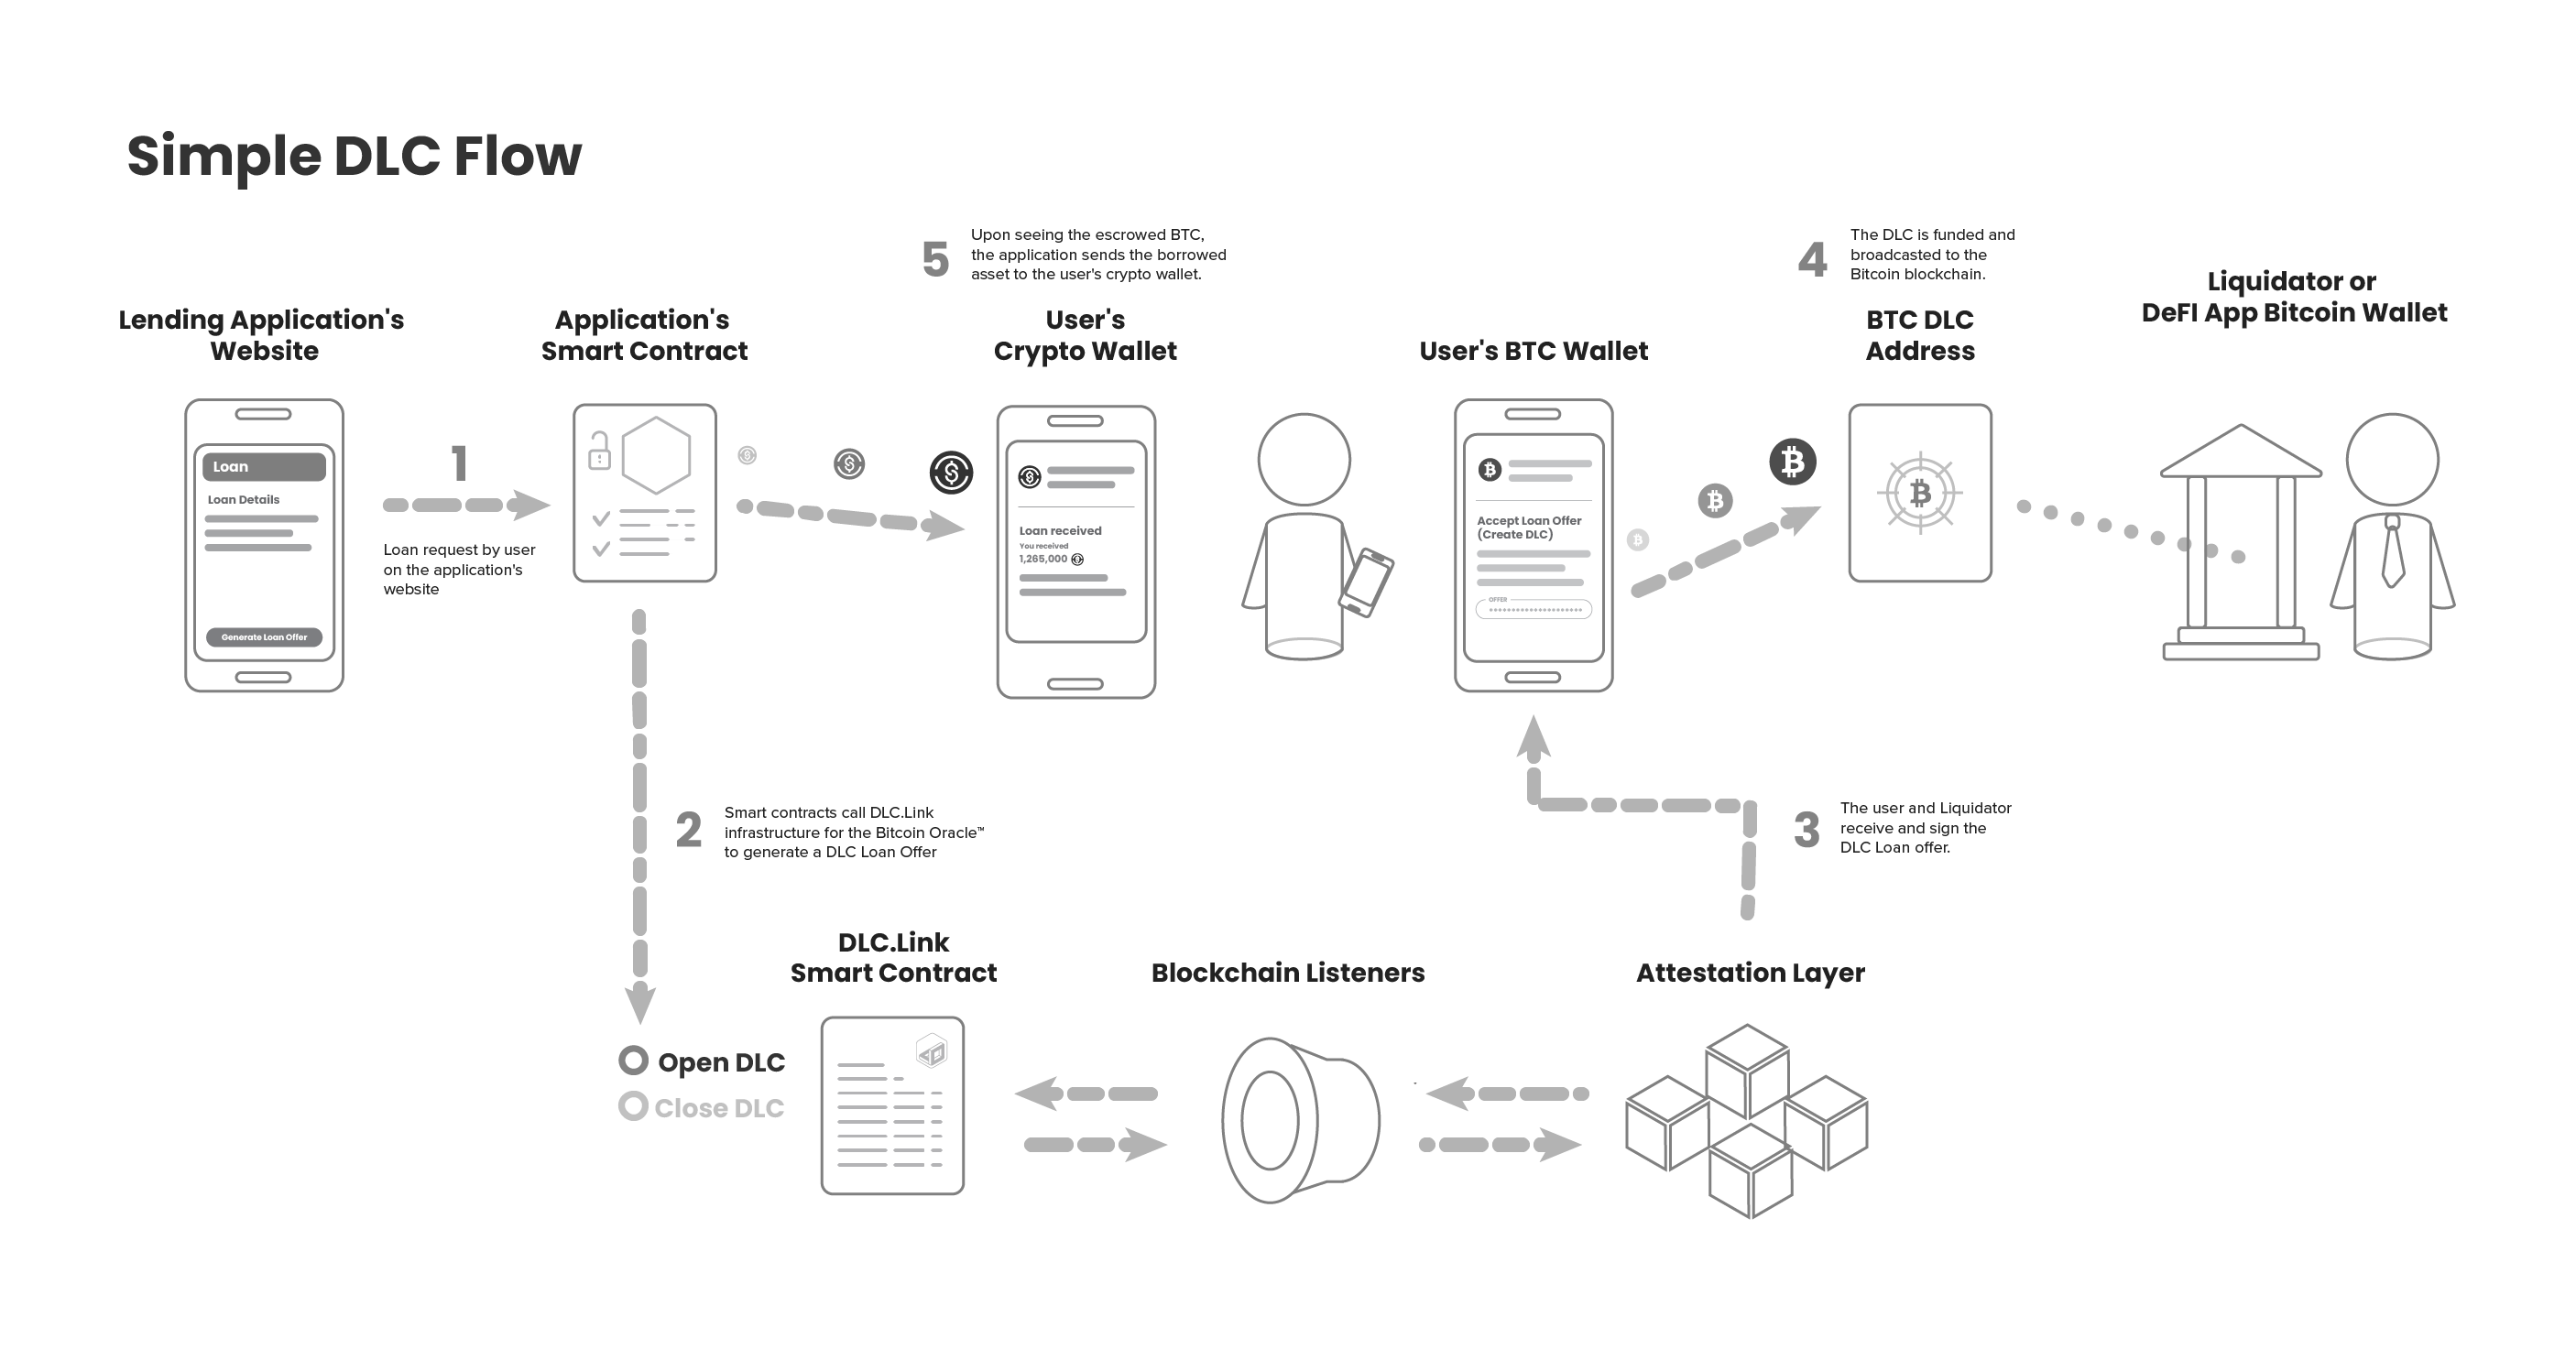
\includegraphics[width=\textwidth]{simple_dlc_flow}
  \end{center}

  \subsection{The Bitcoin Attestor\textsuperscript{TM}}

  The Bitcoin Attestor plays the role of mediator by confirming the outcome for DLC participants. Often multiple oracles will be involved in a single contract (DLC), which can require an m-of-n consensus among the selected oracles. DLC.Link’s Bitcoin Attestor\textsuperscript{TM} cryptographically attests to the outcome of events happening in the real world or on other blockchains.

  The attestation of the Bitcoin Attestor, what data it signs and thus picks the winning outcome from the set of possible outcomes in the DLC, is the most critical piece of data in the process. As a core tenant of web3 infrastructure, it is recommended that a consensus model is used, with multiple Bitcoin Attestors agreeing on an outcome. Any design for determining this outcome via on-chain or off-chain data can be supported by our open-source Bitcoin Attestor model. In the next section, we will detail our current smart contract solution, which allows for complex smart contracts to generate outcomes, which are automatically fed into Bitcoin Attestors and become attested outcomes.

  The reader should keep in mind that although we receive outcomes from fully-featured smart contracts on various chains, the DLC paradigm greatly reduces potential attack vectors. All possible outcomes in a DLC are predetermined upon DLC creation; once BTC is locked in, only the two participants in the DLC are able to receive those funds.

  DLC.Link provides open-source software enabling organizations to easily and safely run their own Bitcoin Attestor and participate in the network.

  \subsection{Smart Contracts}

  Smart contracts are the backbone of the complex thriving ecosystem of DeFi and general web3 development. They communicate between various on-chain sources, including data oracle systems, DeFi/DApp contracts and DLC.Link’s smart contracts. Smart contracts on other blockchains such as Ethereum are not necessary for running DLCs or powering Bitcoin Attestors, as that can be done by any automated data source. But when it comes to programmatically moving currency, the decentralized web is usually the best choice.

  DLC.Link has launched management smart contracts on Ethereum and Stacks and is soon launching on other chains. The DLC.Link contract acts as a communication layer between Bitcoin Attestors and smart contracts, and functions similarly to Chainlink’s direct-request contracts. This contract allows apps to leverage DLCs to move and manage native Bitcoin directly from these chains.

  \subsection{Wallet integration library}

  Signing a DLC requires functionality not yet broadly present in Bitcoin wallets. Therefore, DLC.Link provides open-source libraries and step-by-step guides for easily integrating DLC signing into existing Bitcoin wallets. Current libraries implementing the DLC specification are available in Rust and JavaScript.

  In order to sign a DLC, both participants in the contract need to follow the DLC signing protocol details in the DLC open-source specification.\footnote{\url{https://github.com/discreetlogcontracts/dlcspecs}} This process requires the creation of each outcome’s Schorr signatures to be executed by each party. DLC.Link’s library facilitates DLC signing in wallets.

  To sign successfully, the Bitcoin wallet need not know any complex details that may be behind the DLC, such as details of the DeFi loan on Ethereum. However, the DLC itself contains a minimal set of information – the possible outcomes and amount of BTC being locked in the DLC – which should be shown to the user during contract signing. For an example, see below:

  \begin{figure}[!ht]%
    \centering
    \subfloat{{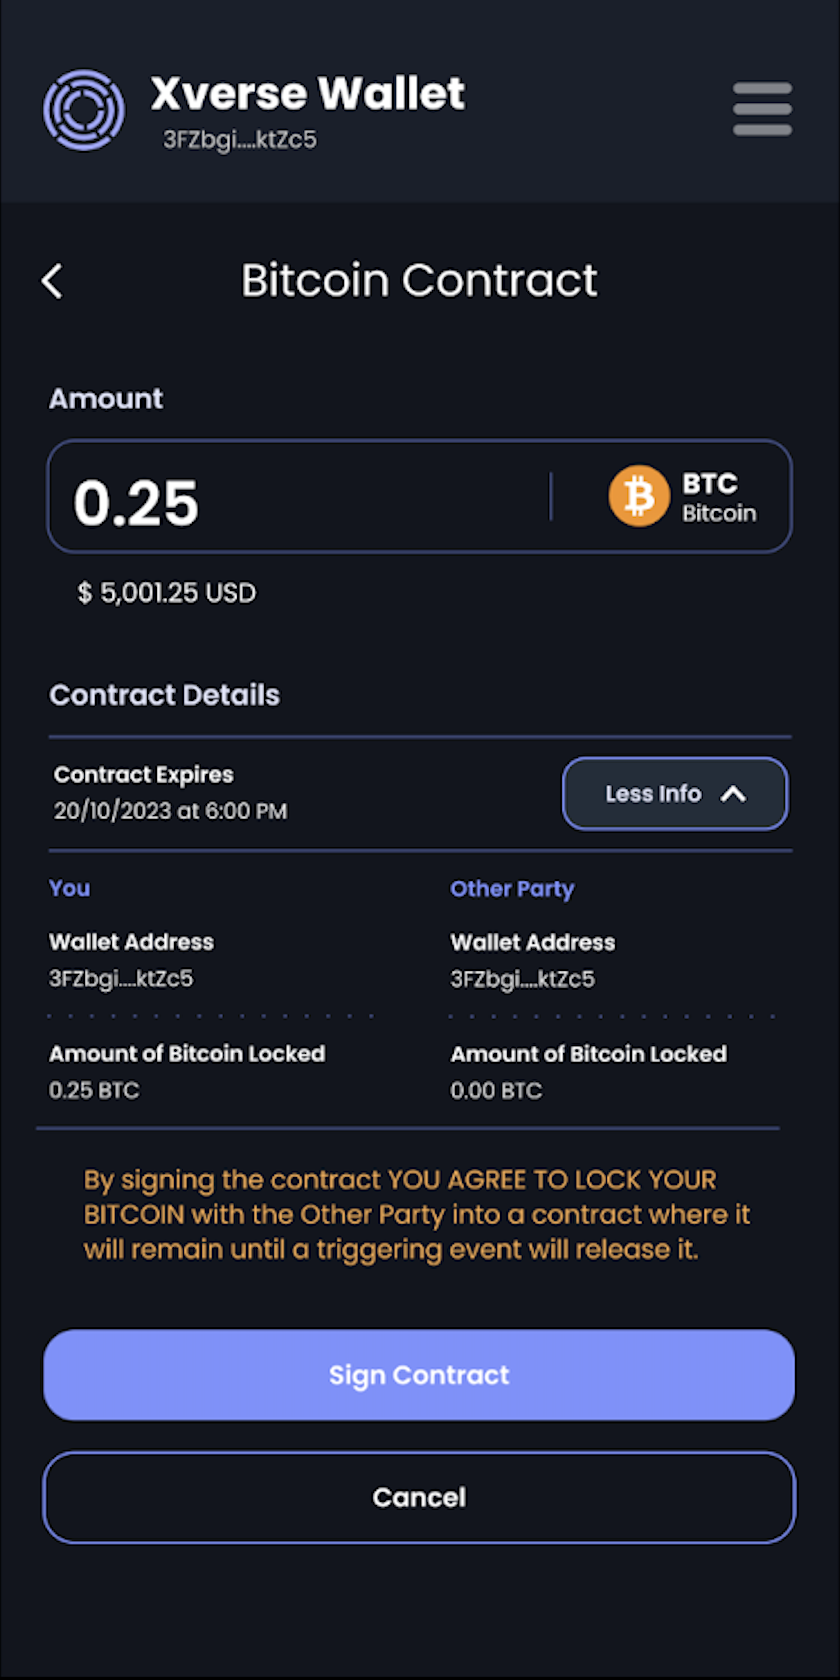
\includegraphics[width=0.32\linewidth]{wallet1} }}%
    \subfloat{{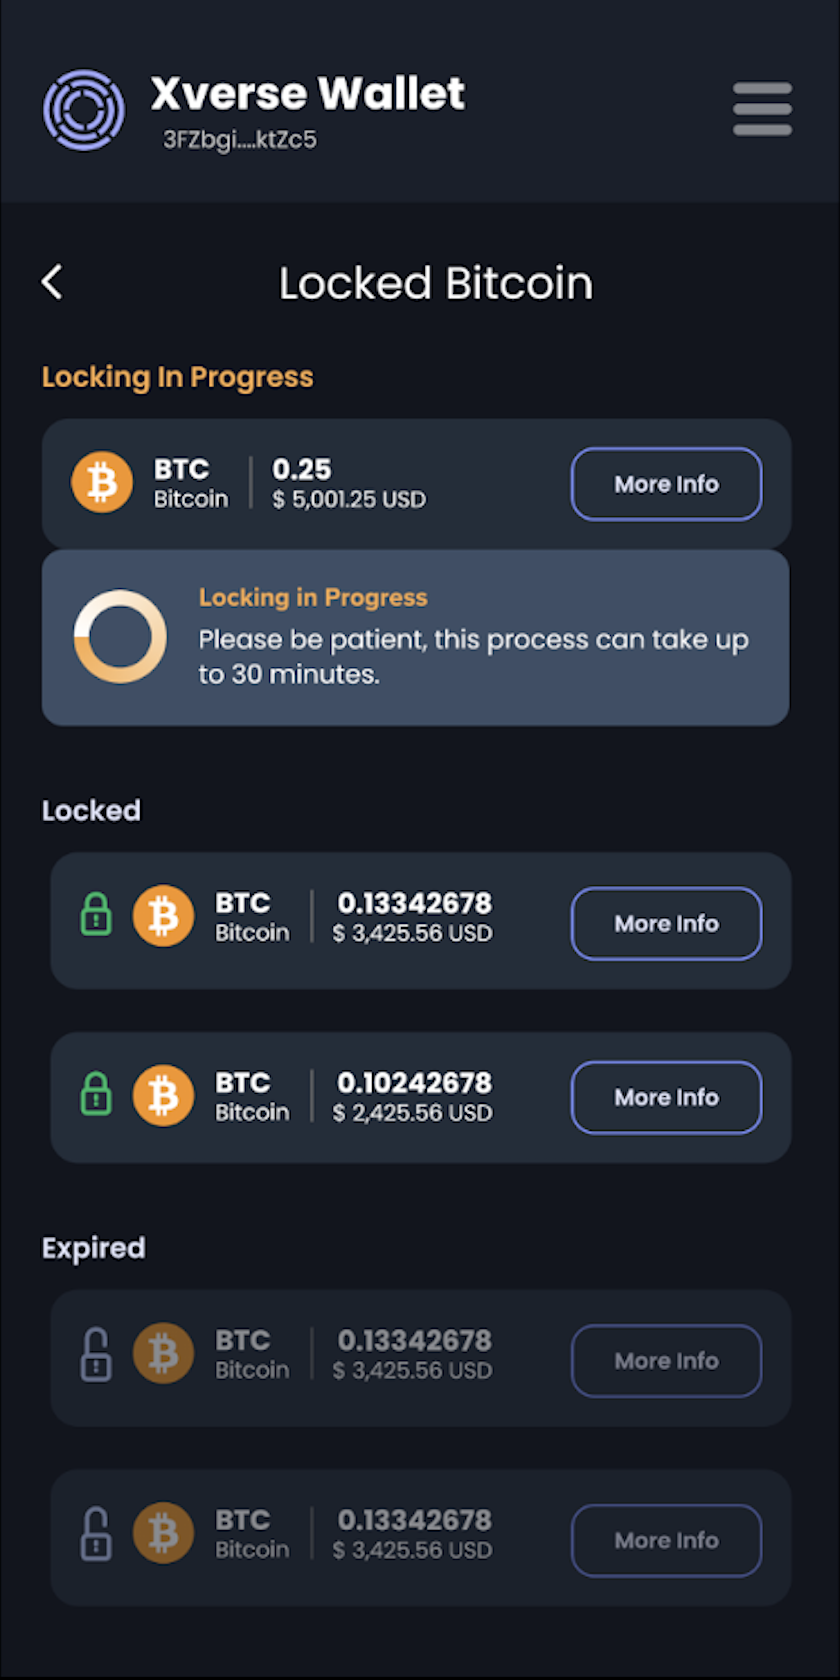
\includegraphics[width=0.32\linewidth]{wallet2} }}%
    \subfloat{{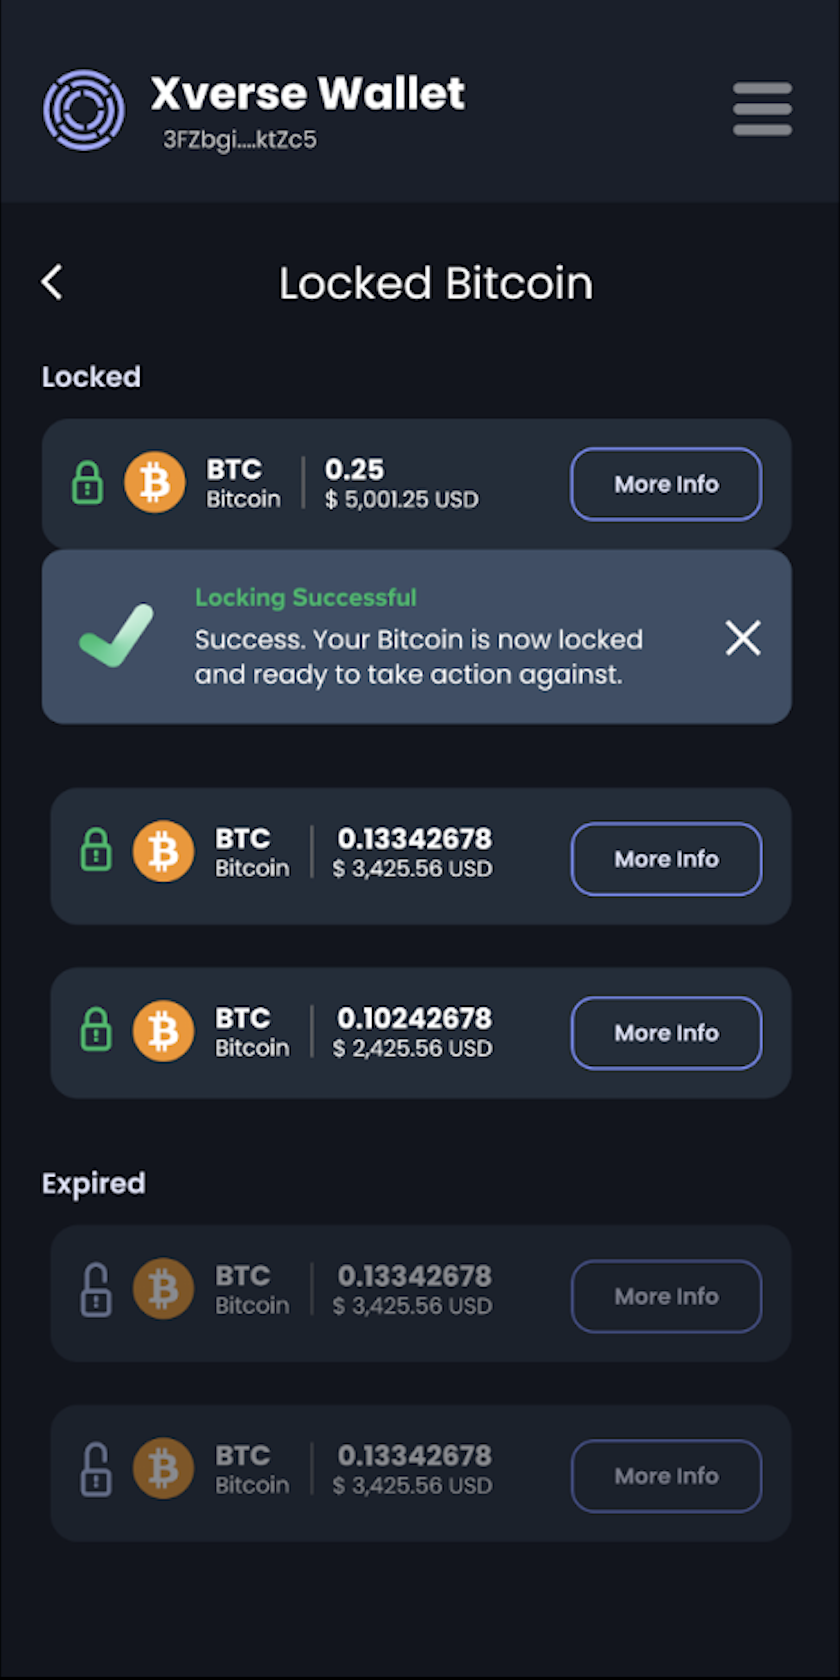
\includegraphics[width=0.32\linewidth]{wallet3} }}%
    \caption{DLC signing in Xverse wallet}%
    \label{fig:example}%
  \end{figure}

  \subsection{Deposit Token}

  Bitcoin deposited in a DLC can be represented on another chain via a token. This can be implemented as an NFT, a soulbound token, a semi-fungible token or another specification.

  Representing locked native Bitcoin on other chains allows for the asset to be represented in the native format of that chain, granting the power of the contracts on that network. For example, the NFTs can be bought and sold on various NFT marketplaces and their ownership can be easily transferred.
  When the NFT is burned, the corresponding DLC is unlocked and the value flows based on which wallet address triggered the burn function. For example, to facilitate trading, the counterparty to the DLC can be a broker who maintains the second wallet. If the NFT is owned/burned by the original participant, it returns value to that participant. If the NFT has since traded ownership and is burned by any other address, the underlying Bitcoin is transferred to the broker who transfers the Bitcoin to its new owner.

  The metadata details of a deposit token representing Bitcoin in a DLC should include the UUID of the DLC in the Bitcoin Attestation Layer, the addresses of the participants in the original DLC, and the amount of BTC locked in the DLC.

  \subsection{Cloud Storage for DLCs}

  One optional component of the DLC architecture is a storage platform for the contract execution transactions (CETs) of the DLCs from the various wallets. CETs are the set of possible outcomes agreed to between the participating wallets. These CETs are not trivially small ($\sim$100KB to 5MB per DLC) and are best stored off-chain for privacy and fee reduction. Nevertheless, it is important to save them in a reliable manner as losing them may prevent a participant being able to sign and close the DLC.

  Therefore, a system will be designed to store the CETs for a given transaction securely in the cloud against a hash of a user’s Bitcoin key, preventing the problem of a potential loss of CETs if a participant were to lose their wallet. To note, similar solutions are being designed for Lighting Network node data and can likely be combined into a similar product.

  \section{What is the Oracle problem and what is DLC.Link’s approach?}

  Bitcoin Attestors enable countless use cases for transactions requiring non-custodial escrow (trustless third-party middleman) and the movement of Bitcoin (capital). Their capacity to allow trustless deposits as well as to integrate with any outside data feed brings an entire new world to Bitcoin’s functionality. While oracles enable blockchains to interact with off-chain data sources, they do not, however, come without risks. One well-known risk is the oracle problem.

  The oracle problem refers to the issue of integrating off-chain data into on-chain smart contracts. Bitcoin transactions, one of the simplest forms of smart contract, typically leverage limited data, including public keys, signatures, timestamps and block sizes. This is reliable as its validity is objective and trustlessly verifiable through the blockchain. Integrating data, for example, like the current price of an asset, into a smart contract in a trustless way poses a challenge. Currently, there are no established methods for ensuring the data provided by either the counterparty or the intermediary is authentic.

  The core question remains how can off-chain data be trusted? As attestors' attestations often come from off-chain sources this is a major concern. If there is only one oracle for a network, this presents a single point of failure. This undermines the true purpose of decentralized applications. This is the crux of the oracle problem. If the Bitcoin oracle goes offline, then data stops flowing on-chain which prevents final settlement on Bitcoin. Worse yet, if the Bitcoin oracle is manipulated, the data sourced from off-chain systems may be compromised. An oracle that publishes incorrect outcomes allows for fraudulent Bitcoin payments to occur defeating the entire purpose of a trustless system.

  DLC.Link has developed a solution to this problem. DLC.Link designed a decentralized network of attestors that listen to events from numerous other blockchains which leverages the trustless and decentralized nature of the greater blockchain ecosystem. DLC.Link combines DLCs with proven oracle solutions like Chainlink in order to unlock Bitcoin liquidity without the need for a trusted third party. To successfully bridge the gap between the strongest, decentralized asset, Bitcoin, and other smart contract blockchains, requires numerous Bitcoin Attestors to mitigate data inaccuracy, collusion, and downtime. DLC.Link is building the infrastructure for anyone to set-up and run a Bitcoin Attestor. As the Bitcoin Attestation Layer\textsuperscript{TM} matures, this will further empower developers and applications on any blockchain or system to accept Bitcoin collateral without any of the implications, restrictions, or risk of using a third-party. Said another way, the combination of DLCs and a Bitcoin Attestation Layer\textsuperscript{TM} remove the need to wrap, bridge, or use CeFi for any BTC related transactions. The DLC.Link infrastructure will serve anyone willing to use BTC as capital for any smart contract conforming to the Bitcoin principle of a trustless monetary system.

  \section{Conclusion}

  Discreet Log Contracts solve the problems plaguing today’s custody, bridging, and CeFi solutions. The market impact of safe lending and finance on Bitcoin cannot be overstated. In the traditional finance world, escrow contracts power the global derivatives market worth over \$1 Quadrillion. DLC.link is helping build a global, decentralized financial system by enabling smart contract applications on every blockchain to use native Bitcoin. We believe that DLCs represent the next generation in Bitcoin utility.

\end{document}
